\section{Newton's Laws of Motion}

\begin{multicols}{2}


\section*{Newton's First Law and Inertia}
\textbf{Newton's First Law: }\emph{An object at rest will remain at rest and an object in motion will remain in motion at a constant speed in a straight line unless acted upon by an external force.}

\subsection{Bucket Swing}

\begin{center}
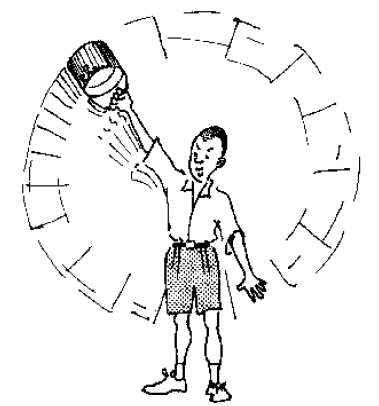
\includegraphics[width=0.4\textwidth]{./img/source/bucket-swing.png}
\end{center}

\begin{description*}
%\item[Subtopic:]{}
\item[Materials:]{Bucket, rope, water}
%\item[Setup:]{}
\item[Procedure:]{Fill a bucket about half way with water and attach a rope to the handle. Swing the rope in a vertical circle so that the bucket is facing downwards at the top of its arc.}
\item[Hazards:]{Don't try to stop the bucket at the top of its swing.}
%\item[Questions:]{}
\item[Observations:]{The water remains in the bucket, even when turned upside-down. You can feel the bucket pulling outwards as you spin it.}
\item[Theory:]{The water and bucket are being pulled outwards by a force known as \emph{centripetal force}. This is essentially a result of the inertia of the items, as they want to continue their motion in a straight line path at any given point throughout the swing. You must constantly exert a force on the rope to cause the bucket to change its direction of motion.}
%\item[Applications:]{}
%\item[Notes:]{}
\end{description*}

\subsection{Card Flick}

\begin{center}
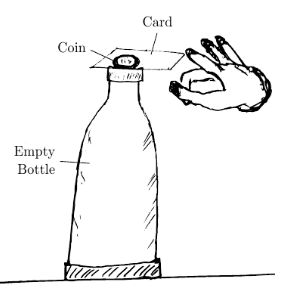
\includegraphics[width=0.35\textwidth]{./img/inertia.png}
\end{center}

\begin{description*}
%\item[Subtopic:]{}
\item[Materials:]{Card, bottle/cup, coin}
%\item[Setup:]{}
\item[Procedure:]{Place the coin on a card so that it rests above the opening of a bottle or cup. Flick the card horizontally.}
%\item[Hazards:]{}
%\item[Questions:]{}
\item[Observations:]{The card goes flying off but the coin drops straight down into the bottle.}
\item[Theory:]{The inertia of the heavy coin is large compared to the friction between the card and coin. Thus it remains in place while the lightweight card flies away.}
%\item[Applications:]{}
\item[Notes:]{The trick works best with a heavy coin and by making sure the card is flicked as horizontally as possible.}
\end{description*}

\subsection{Bucket Pendulums}

\begin{center}
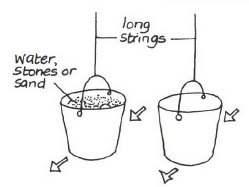
\includegraphics[width=0.4\textwidth]{./img/vso/bucket-pendulums.jpg}
\end{center}

\begin{description*}
%\item[Subtopic:]{}
\item[Materials:]{2 buckets, sand/water/stones, rope}
%\item[Setup:]{}
\item[Procedure:]{Hang two buckets from a support using rope. Fill one with sand, water or some other weight. Try to push each bucket.}
%\item[Hazards:]{}
%\item[Questions:]{}
%\item[Observations:]{}
\item[Theory:]{Inertia must be overcome to start a bucket in motion. The heavier bucket has more inertia and hence requires a greater force to begin swinging.}
%\item[Applications:]{}
%\item[Notes:]{}
\end{description*}

\subsection{Standing Passenger}

\begin{center}
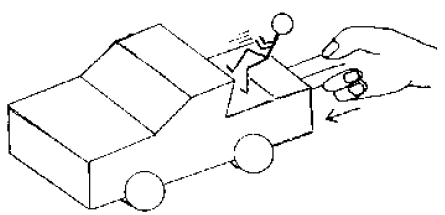
\includegraphics[width=0.45\textwidth]{./img/source/passenger.png}
\end{center}

\begin{description*}
%\item[Subtopic:]{}
\item[Materials:]{Toy car, block of wood}
%\item[Setup:]{}
\item[Procedure:]{Make a toy car out of matchboxes and bottle caps so that there is an open space like the bed of a truck. Stand a tall, thin object such as a block of wood or cardboard passenger in the car. Push the car forward suddenly, make it turn a corner and stop it suddenly.}
%\item[Hazards:]{}
%\item[Questions:]{}
\item[Observations:]{The passenger falls backward when the car moves forward suddenly; falls to the right when the car turns to the left; and falls forward when the car stops suddenly.}
\item[Theory:]{The passenger's inertia wants to keep the passenger at rest or moving in a straight line at constant speed. When the car accelerates, the passenger falls over.}
\item[Applications:]{Standing on a bus}
%\item[Notes:]{}
\end{description*}

\subsection{Spinning Eggs}

%\begin{center}
%\includegraphics[width=0.4\textwidth]{./img/source/.png}
%\end{center}

\begin{description*}
%\item[Subtopic:]{}
\item[Materials:]{1 fresh egg, 1 boiled egg}
%\item[Setup:]{}
\item[Procedure:]{Place the two eggs on a table. Spin the first egg. Stop it briefly with your hand and then release it. Repeat for the second egg and note any differences you observe.}
%\item[Hazards:]{}
\item[Questions:]{Which egg is fresh and which is boiled?}
\item[Observations:]{The fresh egg continues spinning after briefly stopping it, while the boiled egg stops completely.}
\item[Theory:]{The fresh egg contains liquid inside, which continues spinning independent of the egg being stopped, due to its inertia. The boiled egg is solid inside, so it spins as a single unit and stops when the egg is stopped briefly by your hand.}
%\item[Applications:]{}
%\item[Notes:]{}
\end{description*}

%==================================================================================================%

\section*{Newton's Second Law and Momentum}
\textbf{Newton's Second Law:} \emph{The rate of change of momentum of a body is directly proportional to the applied force and takes place in the direction in which the force acts.}\\
\textbf{Force} = mass $\times$ acceleration\\
\textbf{Momentum} = mass $\times$ velocity

\subsection{Atwood's Machine}

%\begin{center}
%\includegraphics[width=0.4\textwidth]{./img/source/.png}
%\end{center}

\begin{description*}
%\item[Subtopic:]{}
\item[Materials:]{\nameref{sec:pulleys}, string, \nameref{sec:masses}, stopwatch, metre rule}
\item[Setup:]{Attach a 1.5 m string to 2 known masses (e.g. 100 g and 90 g). Run the string across the pulley and support the larger mass so that the smaller mass rests on the table. Measure the height $h$ of elevation of the large mass.}
\item[Procedure:]{Release the large mass and use a stopwatch to measure the time taken to reach the table $t$. Repeat 3 or 4 times and take an average reading for time taken. Repeat for different masses.}
%\item[Hazards:]{}
\item[Questions:]{Determine the acceleration of the system using the equation of motion $s=v_0t+\frac{1}{2}at^2$, where $s=h$ and $v_0=0$.}
%\item[Observations:]{}
\item[Theory:]{Newton's Second Law tells us that $F=ma$. Here, $F$ is the net force of gravity acting on the system, and is given by $(m_1-m_2)g$, where $g$ is the gravitational constant. The combined mass of the system is $(m_1+m_2)$, so the acceleration can be given as $a=\cfrac{(m_1-m_2)g}{(m_1+m_2)}$. Calculate the theoretical value of $a$ using this formula, then compare to the experimental value obtained above.}
%\item[Applications:]{}
\item[Notes:]{Use similar masses to get more accurate results.}
\end{description*}

\subsection{Bumping Bottles}

\begin{center}
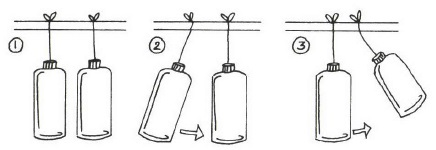
\includegraphics[width=0.49\textwidth]{./img/vso/bumping-bottles.jpg}
\end{center}

\begin{description*}
%\item[Subtopic:]{}
\item[Materials:]{2 bottles, string, horizontal support}
%\item[Setup:]{}
\item[Procedure:]{Hang 2 bottles side by side along a horizontal support. Lift one and release it, noting the effect on the other bottle. Then try varying the masses of the bottles by filling them with different amounts of water and try again.}
%\item[Hazards:]{}
%\item[Questions:]{}
\item[Observations:]{When the bottles are empty, the first one comes to rest after hitting the second, and the second bottle reaches a height similar to the original release height of the first.}
\item[Theory:]{When the bottles touch, momentum is transferred from one to the other. The relative velocities of the bottles, $v_1$ and $v_2$, depend on their relative masses, $m_1$ and $m_2$, according to $m_1v_1 = m_2v_2$. Momentum is conserved.}
%\item[Applications:]{}
%\item[Notes:]{}
\end{description*}

\subsection{Pile of Coins}

%\begin{center}
%\includegraphics[width=0.4\textwidth]{./img/.png}
%\end{center}

\begin{description*}
%\item[Subtopic:]{}
\item[Materials:]{Pile of coins and books}
%\item[Setup:]{}
\item[Procedure:]{Try to remove the bottom book without upsetting the pile. Impossible? To remove the bottom coin from a pile, flick another coin at it.}
%\item[Hazards:]{}
%\item[Questions:]{}
%\item[Observations:]{}
\item[Theory:]{The momentum of the flicked coin is transferred to the bottom of the pile. The momentum overcomes inertia.}
%\item[Applications:]{}
%\item[Notes:]{}
\end{description*}

\subsection{Dropping Fruit}

\begin{center}
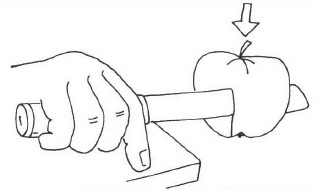
\includegraphics[width=0.35\textwidth]{./img/vso/dropping-fruit.jpg}
\end{center}

\begin{description*}
%\item[Subtopic:]{}
\item[Materials:]{Knife, fruit}
%\item[Setup:]{}
\item[Procedure:]{Drop a fruit onto a sharp knife from different heights.}
%\item[Hazards:]{}
%\item[Questions:]{}
%\item[Observations:]{}
\item[Theory:]{The farther the fall, the greater the momentum and the deeper the cut.}
%\item[Applications:]{}
%\item[Notes:]{}
\end{description*}

%\subsection{Conservation of Linear Momentum}
%
%%\begin{center}
%%\includegraphics[width=0.4\textwidth]{./img/source/.png}
%%\end{center}
%
%\begin{description*}
%%\item[Subtopic:]{}
%\item[Materials:]{}
%\item[Setup:]{}
%\item[Procedure:]{}
%\item[Hazards:]{}
%\item[Questions:]{}
%\item[Observations:]{}
%\item[Theory:]{}
%\item[Applications:]{}
%\item[Notes:]{}
%\end{description*}

%==================================================================================================%

\section*{Newton's Third Law}
\textbf{Newton's Third Law: }\emph{For every action there is an equal and opposite reaction.}

\subsection{Balloon Rocket}

\begin{center}
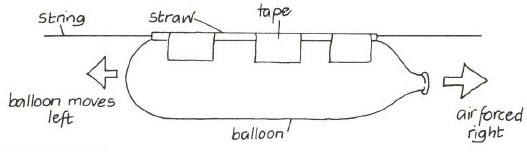
\includegraphics[width=0.49\textwidth]{./img/vso/balloon-rocket.jpg}
\end{center}

\begin{description*}
%\item[Subtopic:]{}
\item[Materials:]{Balloon, string, straw, tape}
%\item[Setup:]{}
\item[Procedure:]{Run a zip line using string between two tables or chairs. Thread a straw and tape it to the balloon so that it can slide across the line. Blow up the balloon and release it to fly across the string.}
%\item[Hazards:]{}
%\item[Questions:]{}
%\item[Observations:]{}
\item[Theory:]{As the air is forced out the opening in the balloon, there is an equal and opposite force applied to the balloon which propels it across the line. This is an application of Newton's Third Law.}
%\item[Applications:]{}
%\item[Notes:]{}
\end{description*}

\subsection{Pushing a Canoe}

\begin{center}
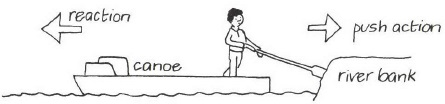
\includegraphics[width=0.49\textwidth]{./img/vso/canoe-push.jpg}
\end{center}

\begin{description*}
%\item[Subtopic:]{}
%\item[Materials:]{}
%\item[Setup:]{}
%\item[Procedure:]{}
%\item[Hazards:]{}
%\item[Questions:]{}
%\item[Observations:]{}
%\item[Theory:]{}
\item[Applications:]{Jet airliners and canoes employ Newton's Third Law. Hot gases are forced out of an airliners engines in one direction (action) - this is known as thrust. The plane moves in the opposite direction (reaction). The canoe also moves away from the push action.}
%\item[Notes:]{}
\end{description*}

\subsection{Boat Thrust}

\begin{center}
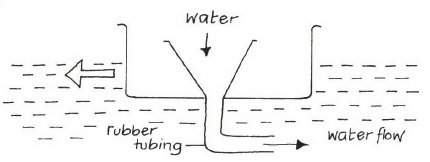
\includegraphics[width=0.45\textwidth]{./img/vso/boat-thrust.jpg}
\end{center}

\begin{description*}
%\item[Subtopic:]{}
\item[Materials:]{Plastic container, rubber tubing, funnel}
\item[Setup:]{Make the tug boat as shown. }
%\item[Procedure:]{}
%\item[Hazards:]{}
%\item[Questions:]{}
\item[Observations:]{As water is poured into the funnel, the boat moves forward.}
\item[Theory:]{Water is forced out the rear tube by gravity (action), which propels the boat forward (reaction).}
\item[Applications:]{Students can compete using different materials to see which travels the fastest.}
%\item[Notes:]{}
\end{description*}

\subsection{Pencil Launch}

\begin{center}
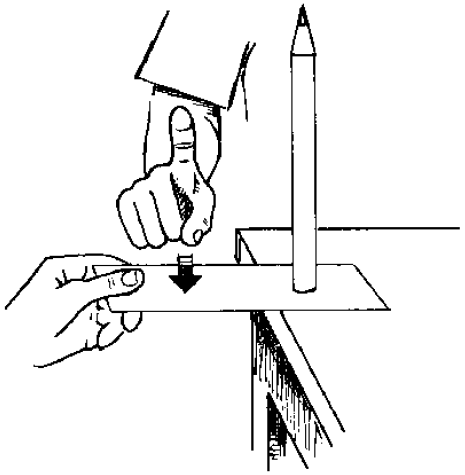
\includegraphics[width=0.33\textwidth]{./img/source/pencil-launch.png}
\end{center}

\begin{description*}
%\item[Subtopic:]{}
\item[Materials:]{Pencil, card}
%\item[Setup:]{}
\item[Procedure:]{Stand a pencil upright on a card at the edge of a table. At once hit the card with your finger so that it leaves the table.}
%\item[Hazards:]{}
%\item[Questions:]{}
\item[Observations:]{Pushing the card downwards (action) causes the pencil to fly upwards (reaction).}
%\item[Theory:]{}
%\item[Applications:]{}
%\item[Notes:]{}
\end{description*}

\columnbreak

\subsection{Elastic Boxes}

\begin{center}
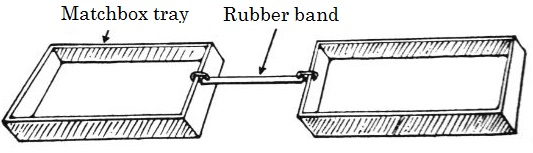
\includegraphics[width=0.45\textwidth]{./img/n3-matchbox.jpg}
\end{center}

\begin{description*}
%\item[Subtopic:]{}
\item[Materials:]{Matchboxes, rubber band, stones}
%\item[Setup:]{}
\item[Procedure:]{Tie or staple each end of the rubber band to a matchbox tray as shown. Pull the trays apart and then release them both at the same time. Now add stones or small nails in one lid and repeat for different weights.}
%\item[Hazards:]{}
%\item[Questions:]{}
\item[Observations:]{When both trays are empty, they pull equally on each other. When stones are added to one, the pull is unequal.}
\item[Theory:]{The stones act with the tray as a single object with more mass, hence it is not pulled as much by the rubber band.}
%\item[Applications:]{}
%\item[Notes:]{}
\end{description*}

\subsection{Matchstick Rocket}

\begin{center}
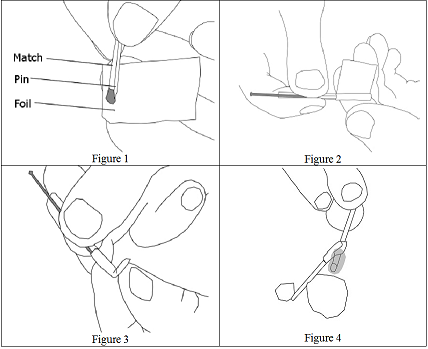
\includegraphics[width=0.45\textwidth]{./img/matchstick-rocket-1.png}
\end{center}

\begin{description*}
%\item[Subtopic:]{}
\item[Materials:]{Matches, aluminum foil, pin/syringe needle}
\item[Setup:]{Rip a small piece of foil about 2 cm $\times$ 3 cm. Hold a pin and match together and wrap the foil tightly around the head of the match so that about 1 cm of foil extends beyond the tip. Fold down the extra foil. Remove the pin by sliding it out the bottom, leaving a thin tunnel. }
\item[Procedure:]{Support the match rocket at a 45$^\circ$ angle on a stone. Light another match and hold it under the foil of the rocket.}
\item[Hazards:]{When igniting, keep your face away from the rocket.}
%\item[Questions:]{}
\item[Observations:]{After a few seconds, the rocket is propelled forward.}
\item[Theory:]{The rocket launches when the match head inside the foil ignites due to the heat of the surrounding foil. The gases are expelled backwards through the thin tunnel (action), and the rocket is driven forward (reaction) by an equal and opposite force.}
%\item[Applications:]{}
%\item[Notes:]{}
\end{description*}

\vfill
\columnbreak

\subsection{Candle Boat}

\begin{center}
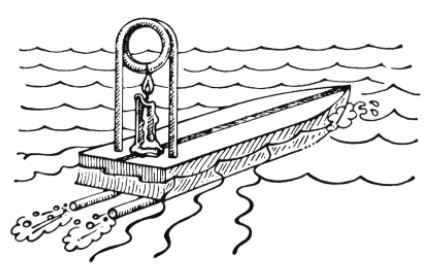
\includegraphics[width=0.4\textwidth]{./img/candle-boat.jpg}
\end{center}

\begin{description*}
%\item[Subtopic:]{}
\item[Materials:]{Candle, wood block, copper tube, basin of water}
\item[Setup:]{Make a small boat using a wood block or plastic/tin container. Insert a loop of copper tubing as shown.}
\item[Procedure:]{Fill the tube with water and place the boat in a large container of water. Set a lit candle under the loop of the tubing.}
%\item[Hazards:]{}
%\item[Questions:]{}
%\item[Observations:]{}
\item[Theory:]{As the water is heated inside the loop, it is driven out of one side of the tubing. The backward motion of the water causes the boat to move forward.}
%\item[Applications:]{}
%\item[Notes:]{}
\end{description*}

\subsection{Bottle Rocket}

%\begin{center}
%\includegraphics[width=0.4\textwidth]{./img/source/.png}
%\end{center}

\begin{description*}
%\item[Subtopic:]{}
\item[Materials:]{500 mL bottle, nail, rubber stopper, pin, ball/bicycle pump, tape, pen tube, rigid straight wire (bicycle spoke), water}
\item[Setup:]{Heat a nail and poke a hole in the bottle lid. Cut a round rubber stopper to fit this hole. Pierce the stopper with the needle of the bicycle pump and insert it in the bottle top. Cut a hollow pen tube into two pieces and tape to the side of the bottle in a straight line.}
\item[Procedure:]{Insert the rigid wire into the ground outside. Fill the bottle half way with water and tighten the lid. Mount the pen tube supports on the rigid wire. Insert the bicycle pump needle through the stopper in the lid and pump until the stopper is pushed out completely.}
\item[Hazards:]{Make sure no one is standing in the way of the rocket. Launch in a large open space.}
%\item[Questions:]{}
\item[Observations:]{When the stopper is forced out of the bottle the rocket flies into the air.}
\item[Theory:]{When the stopper leaves the bottle, pressurized air forces water out of the bottom of the bottle at a high speed. This results in a forward reaction force on the rocket.}
%\item[Applications:]{}
%\item[Notes:]{}
\end{description*}

%==================================================================================================%

% NOT USED
%
%
%\subsection{Conservation of Linear Momentum}
%
%\subsubsection*{Learning Objectives}
%\begin{itemize}
%\item{To demonstrate the principle of conservation of linear momentum}
%\end{itemize}
%
%\subsubsection*{Background Information}
%Everything has momentum which depends on its mass and velocity.  
%$$\mathrm{momentum} = \mathrm{mass} \times \mathrm{velocity}$$ 
%The momentum of an individual body can change as its velocity or mass changes. However, if two objects collide, the total momentum of the objects is conserved.  This means that the total momentum of the objects before the collision is equal to their total momentum after the collision.
%
%\subsubsection*{Materials}
%Toy car with motor, plane surface or smooth table, metre rule or tape measure, beam balance*, different sized stones, and stop watch
%
%\subsubsection*{Preparation Procedure}
%\begin{enumerate}
%\item{Measure the masses of different stones on the beam balance.}
%\item{Measure the mass of the toy car.}
%\item{Measure a distance of 2~m on the plane surface or table.}
%\item{Make a mark at 0~m and place an obstacle at 2~m.}
%\end{enumerate}
%
%\subsubsection*{Activity Procedure}
%\begin{enumerate}
%\item{Place the toy car at the 0~m mark on the table.}
%\item{Release the car and start your stop watch.}
%\item{Record the time it takes for the car to move from the 0 m mark to the obstacle at the 2 m mark.}
%\item{Use this time and distance to calculate the average velocity of the car.}
%\item{Place a stone on top of the toy car (use tape or string if necessary in order to secure it).}
%\item{Measure the new mass of the car with the stone on top.}
%\item{Start the car and release it on the table at the 0 m mark.}
%\item{Again, measure the time it takes for the car to reach the obstacle at the 2 m mark.}
%\item{Calculate the average velocity of the car and stone.}
%\item{Repeat these steps for various stones, measuring the masses and average velocities for each case.}
%\item{For each case, calculate the momentum of the car and stone.}
%\item{Record your results in a table.  Fill in values for mass, time, velocity and momentum.}
%\item{Compare the values for momentum.}
%\end{enumerate}
%
%\subsubsection*{Results and Conclusions}
%The momentum for each experiment is almost the same.  As the mass increases, the velocity decreases.  However, the product of the two remains the same.  However, the momentum decreases slightly more than expected with increased mass because friction on the axles of the car is also increased.
%When two bodies, one heavy and one light, are acted upon by the same force for the same amount of time, the lighter object's velocity increases more than that of the heavy object.  However, the momentum that each gains is the same.
%
%\subsubsection*{Clean Up Procedure}
%Return all materials to their proper places.
%
%\subsubsection*{Discussion Questions}
%\begin{enumerate}
%\item{What factors affect the momentum of the car?}
%\item{When the mass of the car is increased by adding stones, what happens to the average velocity?}
%\item{What do you observe when comparing the values for momentum?}
%\end{enumerate}
%
%\subsubsection*{Notes}
%Conservation of momentum is only true in a frictionless environment.  However, the effects can be seen clearly even if friction is present.  The toy car has friction between its wheels and axles, so adding mass to the car will increase the effect of friction.  However, it will still be seen that the momentum is relatively equal for each mass.

\end{multicols}

\pagebreak